\documentclass[tikz,border=10pt]{standalone}
\usepackage{amsmath}
\usetikzlibrary{arrows.meta, positioning, calc, decorations.pathreplacing}
\definecolor{c1}{HTML}{000000}
\definecolor{c2}{HTML}{233D4D}
\definecolor{c3}{HTML}{FE7F2D}
\definecolor{c4}{HTML}{EAECF0}
\definecolor{axiscolor}{HTML}{333333}
\definecolor{labelcolor}{HTML}{5F6B75}
\begin{document}
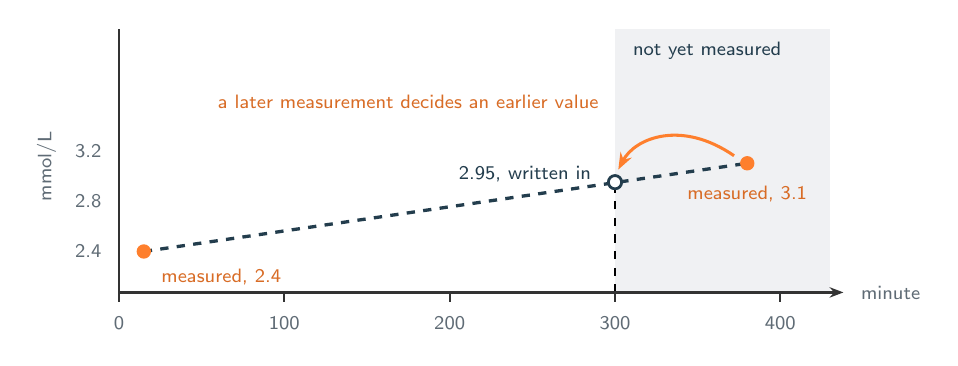
\begin{tikzpicture}[
    every node/.style={font=\sffamily},
    lab/.style={font=\sffamily\scriptsize, text=labelcolor},
    tag/.style={font=\sffamily\scriptsize, text=c2},
    hot/.style={font=\sffamily\scriptsize, text=c3!85!black},
]
\def\X#1{1.40 + #1*0.02100}
\def\Y#1{1.70 + (#1-2.2)*1.60}

% the future, shaded
\fill[c2!07] ({\X{300}}, 1.50) rectangle ({\X{430}}, 4.85);
\node[tag, anchor=north west] at ({\X{305}}, 4.80) {not yet measured};

\draw[axiscolor, line width=0.7pt] (1.40, 1.50) -- (1.40, 4.85);
\foreach \v in {2.4, 2.8, 3.2}{
    \node[lab, anchor=east] at (1.30, {\Y{\v}}) {\v};
}
\node[lab, rotate=90] at (0.48, 3.10) {mmol/L};

% the straight line the imputation draws
\draw[c2, line width=1.2pt, dashed] ({\X{15}}, {\Y{2.4}}) -- ({\X{380}}, {\Y{3.1}});

\fill[c3] ({\X{15}}, {\Y{2.4}}) circle (2.6pt);
\node[hot, anchor=west] at ({\X{15}+0.10}, {\Y{2.4}-0.32}) {measured, 2.4};
\fill[c3] ({\X{380}}, {\Y{3.1}}) circle (2.6pt);
\node[hot, anchor=north] at ({\X{380}}, {\Y{3.1}-0.16}) {measured, 3.1};

% the imputed value at minute 300
\draw[c1, line width=0.8pt, dashed] ({\X{300}}, 1.50) -- ({\X{300}}, {\Y{2.95}});
\fill[white] ({\X{300}}, {\Y{2.95}}) circle (2.4pt);
\draw[c2, line width=1.0pt] ({\X{300}}, {\Y{2.95}}) circle (2.4pt);
\node[tag, anchor=east] at ({\X{300}-0.18}, {\Y{2.95}+0.10}) {2.95, written in};

% the leak
\draw[c3, line width=1.1pt, -{Stealth[length=6pt]}]
    ({\X{372}}, {\Y{3.16}}) .. controls ({\X{340}}, {\Y{3.45}})
    and ({\X{312}}, {\Y{3.30}}) .. ({\X{302}}, {\Y{3.05}});
\node[hot, anchor=south east] at ({\X{296}}, {\Y{3.46}})
    {a later measurement decides an earlier value};

\draw[axiscolor, line width=0.8pt, -{Stealth[length=5pt]}] (1.40, 1.50) -- (10.60, 1.50);
\foreach \m in {0, 100, 200, 300, 400}{
    \draw[axiscolor, line width=0.7pt] ({\X{\m}}, 1.50) -- ({\X{\m}}, 1.38);
    \node[lab, anchor=north] at ({\X{\m}}, 1.32) {\m};
}
\node[lab, anchor=west] at (10.70, 1.50) {minute};
\end{tikzpicture}
\end{document}
